% !TeX spellcheck = sk_SK

%%%%%%%%%%%%%%%%%%%%%%% file typeinst.tex %%%%%%%%%%%%%%%%%%%%%%%%%
%
% This is the LaTeX source for the instructions to authors using
% the LaTeX document class 'llncs.cls' for contributions to
% the Lecture Notes in Computer Sciences series.
% http://www.springer.com/lncs       Springer Heidelberg 2006/05/04
%
% It may be used as a template for your own input - copy it
% to a new file with a new name and use it as the basis
% for your article.
%
% NB: the document class 'llncs' has its own and detailed documentation, see
% ftp://ftp.springer.de/data/pubftp/pub/tex/latex/llncs/latex2e/llncsdoc.pdf
%
%%%%%%%%%%%%%%%%%%%%%%%%%%%%%%%%%%%%%%%%%%%%%%%%%%%%%%%%%%%%%%%%%%%
\documentclass[runningheads,a4paper]{llncs}
\usepackage{dcolumn}
\usepackage{amssymb}
\setcounter{tocdepth}{3}
\usepackage{graphicx}
\usepackage{epstopdf}
\usepackage[slovak]{babel}
\usepackage[utf8]{inputenc}
\usepackage[bottom]{footmisc}

\usepackage{url}
\begin{document}
\title{Predikcia popularity článkov}
\subtitle{Objavovanie znalostí}
\titlerunning{Predikcia popularity článkov}
\author{Martin Číž, Peter Uherek}
\institute{Fakulta informatiky a informačných technológií,\\
Slovenská technická univerzita}
\authorrunning{Predikcia popularity článkov}
\maketitle

\begin{abstract}
  Našou úlohou je zostrojiť model predikcie popularity článkov na základe spravodajských článkov, ktoré sú v textovej podobe.
  Popularita článkov je z pohľadu času nestála. Inú popularitu môže mať článok hodinu od vydania a inú deň po vydaní.
  V našom kontexte chápeme popularitu ako počet všetkých jedinečných prístupov k článku v určitej dobe od jeho vydania.
  Na začiatku sa pokúšame texty jednotlivých získan-ých článkov premeniť na vektor termov, text preto spracovávame vo fázach odstraňovanie stop slov a lematizácia.
  Pre predikovanie počtu prístupov používame metódy regresie v strojovom učení.
  Zaujímavý vplyv na popularitu článku má samotný text článku, názov článku alebo dĺžka článku, preto sa zameriavame na skúmanie vplyvu týchto faktorov na samotnú popularitu článkov.
  Experimentom demonštrujeme použitie spo-mínaných metód, pričom poukazujeme na bariéry, ktoré nám bránia v presnom zmeraní predikcie.
  Príkladom je neproporcionálne rozloženie článkov po zoradení do rebríčka popularity - existuje veľa priemerných a slabšie čítaných článkov a len malá množina článkov získava veľkú popularitu.
\end{abstract}

\section{Úvod}
  V súčasnosti sa na webe takmer všetko podriaďuje analytike, čítanosti a 
návštev-nosti s cieľom udržať na svojom webovom sídle čo najviac používateľov na 
čo najdlhší čas. Prevádzkovatelia portálov, ktoré prinášajú rozsiahly a 
dynamický informačný obsah (typicky internetové vydania novín, týždenníkov) 
disponujú veľkým množstvom sekvenčných dát, ktoré zachytávajú správanie sa 
používateľov, históriu ich postupného prechádzania danej webovej lokality. 
Taktiež uchovávajú informácie o svojich článkoch, či už je to samotný názov, 
obsah, dátum vydania alebo téma, ktorej sa článok venuje. Z týchto dát je možné 
nielen spätné vyhodnocovanie čítanosti jednotlivých článkov, ale napr. aj 
predpovedanie popularity jednotlivých článkov či tém, čo môže následne ovplyvniť 
rozloženie webovej stránky. 

\section{Opis dát}
V rámci diplomovej práce sme od vedúceho obdržali z časti predspracované dáta z 15-dňového dumpu internetového vydania denníka SME.
Dáta sú zozbierané z obdobia 7.10. 2009 až 21.10. 2009.
Pôvodný dump obsahuje iba jednu tabuľku, v ktorej sa nachádzajú údaje prístupov používateľov na články stránky sme.sk.
Tieto dáta sú rozšírené v diplomovej práci Pavla Sopka \cite{diplomovka} o ďalších 5 tabuliek, ktoré obsahujú rozšírené dáta o článkoch.
Pre naše potreby tieto rozšírené dáta používame v rámci uľahčenia fázy predspracovania.
Najzaujímavejšie z týchto dát sú dve tabuľky a to tabuľka {\em visits} a tabuľka {\em articles}.

Tabuľka {\em visits} obsahuje vyčistené dáta pôvodného dumpu a je tvorená nasledovnými stĺpcami:
\begin{itemize}
\renewcommand{\labelitemi}{$\bullet$}
  \item Časová pečiatka vytvorenia záznamu.
  \item Cookie používateľa, ktorou identifikujeme či sa jedná o toho istého používateľa.
  \item IP adresa používateľa.
  \item ID článku, na ktorý používateľ pristupoval.
  \item ID miesta alebo článku odkiaľ používateľ pristupoval.
  \item Dostupné informácie o prístupe používateľa (počítač, mobil, tablet).
  \item Lokácia odkiaľ používateľ pristupoval (mesto, štát).
\end{itemize}

Tabuľka {\em articles} je tvorená informáciami o článkoch a má nasledovné stĺpce:
\begin{itemize}
\renewcommand{\labelitemi}{$\bullet$}
  \item ID sekcie a ID kategórie.
  \item Titulok článku.
  \item Obsah článku s html značkami.
  \item Obsah článku bez html značiek (čistý text).
  \item Lematizovaný titulok článku.
  \item Lematizovaný obsah článku.
  \item Hodnota všetkých lematizovaných slov z metódy TFI-DF.
  \item Počet všetkých návštev (nie unikátnych).
  \item Dátum publikovania.
\end{itemize}

\section{Práce iných autorov}
Naším prvým zdrojom je diplomová práca od Pavla Sopka \cite{diplomovka}. 
Práca nás bližšie oboznamuje s postupom spracovania slovenského textu ako je odstraňovanie stop slov, odstránenie interpunkčných znamienok, lematizácia, či hľadanie prídavných mien medzi slovami.

Predpoveďou popularity podobne ako my sa zaoberá aj článok \cite{pulse}. Základne otázky, ktoré tento článok rozoberá, sú:
\begin{itemize}
\renewcommand{\labelitemi}{$\bullet$}
  \item Ovplyvňuje kategória článku jeho populárnosť?
  \item Uprednostňujú čitatelia fakty, alebo preferujú citovo zafarbený text?
  \item Má zmienka slávnej osoby vplyv na popularitu? Závisí to od autora článku?
\end{itemize}
Článok skúma predpovedanie popularity článkov ešte pred ich vydaním. Vytvorí sa viacrozmerný priestor na základe viacerých vlastností článku a odhaduje sa úspešnosť tých vlastností, na základe ktorých sa určuje populárnosť. Práca používa regresné aj klasifikačné metódy strojového učenia.

Článok \cite{topic} sa venuje výberom populárnych článkov na titulnú stranu, pričom používa modelovanie podľa témy (angl. topic modeling).
Práca konštatuje, že odporúčanie dôležitých novinových článkov z veľkej sady je v prípade použitia len obsahu článkov ťažkou úlohou.

\section{Predspracovanie}
% Predspracovanie a výber atribútov: použité metódy, zdôvodnenie
Veľká časť z dát už bola predspracovaná, ale i napriek tomu niektoré stĺpce neobsahujú požadované hodnoty a je potrebné ich dodatočne dopracovať.
Jedným z takýchto stĺpcov je stĺpec lematizovanej titulky a obsahu článku v tabuľke {\em articles}.
Z celkového počtu 151.577 článkov bolo lematizovaných iba 49.300 (33 \%) článkov a nelematizovaných 102.277 (67 \%) článkov.
Pre naše potreby nám tento počet pôvodne lematizovaných článkov nestačí, keďže väčšina týchto článkov nebola vydaná v čase zbierania datasetu a z toho dôvodu ich nemôžeme použiť.
Preto bolo potrebné nájsť spôsob ako lematizovať ostatné články.

Pre lematizáciu článkov sme navrhli skript, ktorý každý obsah článku upraví v nasledovnej postupnosti:
\newline
\newline
text bez html značiek $\rightarrow$ text bez interpunkčných znakov $\rightarrow$ text bez stop slov $\rightarrow$ lematizovaný text $\rightarrow$ lematizovaný text bez stop slov
\newline

Pred lematizáciou odstraňujeme stop slová, aby sme do lematizátora podávali čo najmenší počet slov.
Na samotnú lematizáciu článkov sme použili voľne dostupnú web službu našej fakulty - lemmatizer\footnote{Dostupný na \url{http://text.fiit.stuba.sk/lemmatizer/index.html (2015).}}.
Lematizér sme použili s nastavením rýchlej lematizácie, kde výstupom je čistý text obsahujúci najpravdepodobnejšie lemy oddelené medzerami.

V nasledujúcich riadkoch je uvedený príklad lematizovaného textu po odstránení stop slov:

\begin{multicols}{2}
Pred: Minulý rok si študenti Gymnázia na Grösslingovej ulici založili Gamčácke divadlo ochotníkov. V krátkom čase debutovali komédiou MAThRIX a vďaka jej úspechu sa divadlo rozhodlo pripraviť ďalší projekt. Predstavili ho už v uplynulú sobotu v DK Lúky premiéru mala ich nová komédia Taká obyčajná mafia.

Po: minulý rok študent gymnázium grösslingovej ulica založiť gamčácke divadlo ochotník krátky čase debutovať komédia mathrix vďaka úspech divadlo rozhodnúť pripraviť ďalší projekt predstaviť uplynulý sobota dk lúka premiéra mala nový komédia obyčajná mafia
\end{multicols}

Po lematizácií opätovne odstraňujeme stop slová, ktoré neboli zachytené pred lematizáciou a po lematizácií môžu byť nájdene v zozname stop slov.
Ako zoznam stop slov sme použili voľne dostupný projekt na Google\footnote{Dostupný na \url{https://code.google.com/p/stop-words/source/browse/trunk/stop-words/stop-words/stop-words-slovak.txt?spec=svn3&r=3} (2015).}, ktorý však bolo nutné ručne doplniť o desiatky slov.
Procesom lematizácie neprešlo 1555 článkov z dôvodu neznámeho kódovania na strane databázy. Všetky ostatné články sme po procese lematizácie uložili do databázy.  

Ako bolo spomínané v úvode, popularitu článku nemôžeme empiricky zhodnotiť bez určeného časového obdobia (po jednej hodine sa článok nemusí ešte uchytiť, po jednom dni už môže článok stagnovať na popularite).
Väčšina článkov nadobúda po zverejnení kopček (angl. peak) maximálnych čítaní v krátkom čase, po ktorom začína čítanosť rýchlo stagnovať a zvyšuje sa už len o priemerné hodnoty.
Vytvorili sme si pre články ich priebeh zvyšujúceho sa počtu návštev v čase a na základe neho sme stanovili, že budeme brať počet navštívení článku 24 hodín po jeho vydaní.
Z optimalizačných dôvodov sme si počty vypočítali a pripísali do nového stĺpca v tabuľke s článkami.

\section{Viacnásobna linerárna regresia a spôsob jej vyhodnotenia}
%    DM metódy: stručný opis, zdôvodnenie výberu
Vzhľadom na to, že chceme skúmať závislosť popularity od obsahu článku, sme sa rozhodli použiť viacnásobnú lineárnu regresiu, ktorá skúma lineárnu závislosť medzi dvoma a viacerými premennými. Viacnásobná lineárna regresia sa dá vyjadriť vzorcom: 
\begin{displaymath}
y_i = a_0 + a_1x_{1i} +  a_2x_{2i} \ldots + a_nx_{ni},
\end{displaymath}
kde $y_{i}$ predstavuje predikovaný atribút, v našom prípade počet unikátnych návštev za 24 hodín pre $i$-ty článok. Tento atribút sme pred aplikovaním v viacnásobnej lineárnej regresie previedli do logaritmického tvaru z dôvodu veľkých rozdielov medzi jednotlivými hodnotami návštevnosti článkov.

Atribúty $x_{ij}$ predstavujú číselný vektor pre slová v článkoch získaných z korpusu všetkých článkov pomocou metódy TF-IDF. Číselné hodnoty $x_{ij}$ predstavujú dôležitosť slov, resp. výskyt slov. Hodnota $x_{ij}$ slova pre daný článok $i$ sa zvyšuje úmerne s počtom výskytov slova v dokumente, ale je kompenzovaná frekvenciou slova v korpuse. Frekvencia nám pomáha odhaliť slová, ktoré sa objavujú častejšie a tým pádom sú všeobecnejšie. Príkladom takýchto slov sú prídavné mená. Hodnota $a_j$ predstavuje regresný koeficient pre $j$-ty atribút.

Na vyhodnotenie metódy používame krížovú validáciu. Jej princíp spočíva v rozdelení datasetu na K vzoriek (angl. folds), ktoré sú v ideálnom prípade tvorené rovnakým počtom článkov. Následne prebehne algoritmus K-krát, pričom vždy je jedna vzorka testovacia, zatiaľ čo všetky ostatné vzorky slúžia na trénovanie.

Výsledky krížovej validácie sme verifikovali pomocou chyby predikcie krížovej validácie (angl. Cross-validation error estimate) (CV), ktorá sa vypočíta ako suma chýb predikcie zo všetkých vzoriek. Túto hodnotu dostaneme pomocou vzorca: 
\begin{displaymath}
CV_K = \sum_{k=1}^K \frac{n_k}{n} MSE_k,
\end{displaymath}
kde $K$ je počet vzoriek, $n$ je počet všetkých článkov a $n_k$ je počet článkov vo vzorke $k$. $\frac{n_k}{n}$ predstavuje vážený priemer pre každú vzorku, ktorú je nutné zohľadniť pretože nie každá vzorka môže mať rovnaký počet článkov. V prípade, že má každá vzorka rovnaký počet článkov, vážený priemer je predstavovaný hodnotou $\frac{1}{k}$. $MSE_k$ predstavuje strednú kvadratickú chybu vzorky $k$, ktorá sa vypočíta pomocou vzorca:
\begin{displaymath}
MSE_k = \frac{\sum_{i \in C_k}(y_i-\hat{y_i})^2}{n_k},
\end{displaymath}
kde $y_i$ je pôvodná návštevnosť a $\hat{y_i}$ je predikovaná návštevnosť. Rozdiel medzi týmito dvomi hodnotami je chyba predikcie.

Okrem CV sme úspešnosť viacnásobnej lineárnej regresie hodnotili aj pomocou priemernej chyby predikcie a pomocou mediánu chyby predikcie. Tieto hodnoty boli vypočítané zo všetkých chýb predikcie naraz.

\section{Experimentovanie}
% vyhodnotenie: vyhodnotenie výsledkov, porovnanie metód (aj s publikovanými prácami) a náčrt ďalšieho vhodného smerovania projektu
Viacnásobná lineárna regresia a krížová validácia bola aplikovaná v jazyku R pomocou metódy {\em cvlm}, ktorá sa nachádza v balíčku DAAG. Táto metóda sama rozdelila dáta do viacerých vzoriek a i sama vypočítala hodnotu CV. 

Články, ktoré sme vybrali do lineárnej regresie boli vydané v 15 dňovom období, z ktorého pochádza dump, ktorý sme mali k dispozícii. Dôvod prečo sme si vybrali iba články, ktoré boli vydané iba v tomto období je taký, že sme potrebovali jednotnú množinu článkov, pri ktorých sme exaktne vedeli určiť ich návštevnosť. Pri článkoch, ktoré boli vydané skôr ako bolo časové obdobie zbierania datasetu sme nemali možnosť ako overiť ich skutočnú návštevnosť po vydaní datasetu. Mohli sme zistiť iba ich návštevnosť v rámci obdobia zbierania dát, čo pre naše potreby nebolo vhodné.

Počet článkov, ktoré sme mohli použiť bolo 4196. Pre všetky texty týchto článkov sme aplikovali metódu TF-IDF, ktorá nám ku každému článku priradila vektor hodnôt všetkých slov, ktoré sa vyskytovali v textoch článkov. Počet jedinečných slov pre všetky články bol 58 652. Túto hodnotu sme redukovali a zobrali sme iba najdôležitejšie slová, ktoré sa nachádzali v článkoch. V prvom teste sme takto nechali 106 slov, ktoré sme spoločne s návštevnosťou aplikovali v metóde {\em cvlm}, ktorá rozdelila články na 10 vzoriek po 419 článkov. 

\begin{table}
\begin{center}
	\begin{tabular}{|l|c|c|c|}
	\hline
	Vstupné atribúty & CV & Priemerná chyba & Medián chyby \\ \hline \hline
	106 slov & 74 & 1279 & 157 \\ \hline
	404 slov & 26.9 & 1240 & 145 \\ \hline
	1079 slov & 9.88 & 1186 & 132 \\ \hline
	1357 slov & 7.86 & 1151 & 119 \\ \hline
	2649 slov & 7.74 & 909 & 88.1 \\ \hline
	4526 slov & 3.21e+27 & 1.02e+11 & 97.1 \\ \hline
	5006 slov & 7.08e+30 & 3.16e+18 & 120 \\ \hline
	\end{tabular}
\end{center}
\caption{Tabuľka znázorňuje výsledky pre 4196 článkov s postupným pridávaním atribútov, slov, do viacnásobnej lineárnej regresie. }
\end{table}

Výsledky krížovej validácie z prvého experimentu je možné vidieť v tabuľke číslo 1. Hodnoty CV sú uvedené v logaritmickom tvare. Hodnoty premennej chyby a mediánu chyby predikcie sú uvedené v reálnom tvare. Pri prvom experimente pri 4196 článkoch sme mali priemernú chybu predikcie 1279 a medián chyby bol 157. Tieto dve hodnoty nám naznačujú, že náš regresný model pri polovice článkov dokázal uhádnuť ich čítanosť s chybou menšou ako 157. Priemerná chyba je o niečo vyššia čo je spôsobené veľkou rozmanitosťou čítanosti v článkoch.

Presnosť prvého experimentu je taktiež vidieť na obrázku číslo 1, ktorý znázorňuje na $x$-ovej osi predikovanú návštevnosť a $y$-ovej reálnu čítanosť. V ideálnom prípade, keby náš model predikoval návštevnosť so 100 \% úspešnosťou, tak by všetky hodnoty na obrázku museli byť uložené lineárne. V reálnom prípade sú uložené ako je vidieť na obrázku číslo 1. Za povšimnutie stojí desiata vzorka, ktorá je na obrázku znázornená modrou farbou. Táto vzorka sa zjavne vyznačuje veľkým počtom článkov s vysokou návštevnosťou. Väčšina článkov z tejto vzorky je predikovaná veľmi zle, čo je vidieť aj z obrázku ako tieto výsledky vystupujú z hlavného prúdu výsledkov. Tieto predikcie nám značne zhoršujú výsledok.  
  
                 
\begin{figure}[h!]
  \centering  
      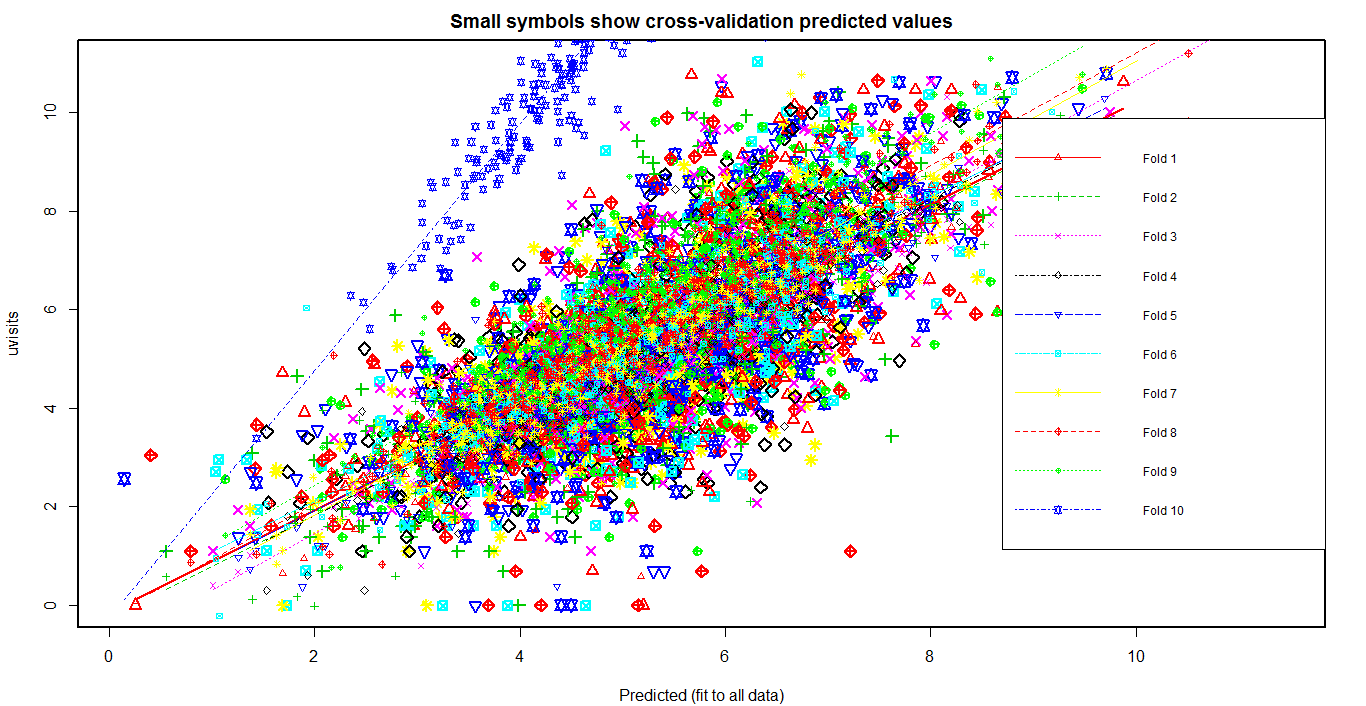
\includegraphics[width=1.0\textwidth]{plot3.png}
  \caption{Obrázok znázorňuje presnosť predikcie pre prvý experiment.}
\end{figure}

Ako je vidieť z tabuľky číslo 1 pri ďalších experimentoch sme pokračovali pridávaním atribútov, slov do viacnásobnej lineárnej regresie. Výsledok sa postupne zlepšoval až sme narazili na taký počet slov, ktorý nám značne zhoršil výsledok. Takýto zlom nastal pri pridaní 4526 slov do modelu. Zmena rozloženia chyb pri postupnom pridávani slov do modelu je vidieť na obrázku číslo 2.

\begin{figure}[h!]
  \centering  
      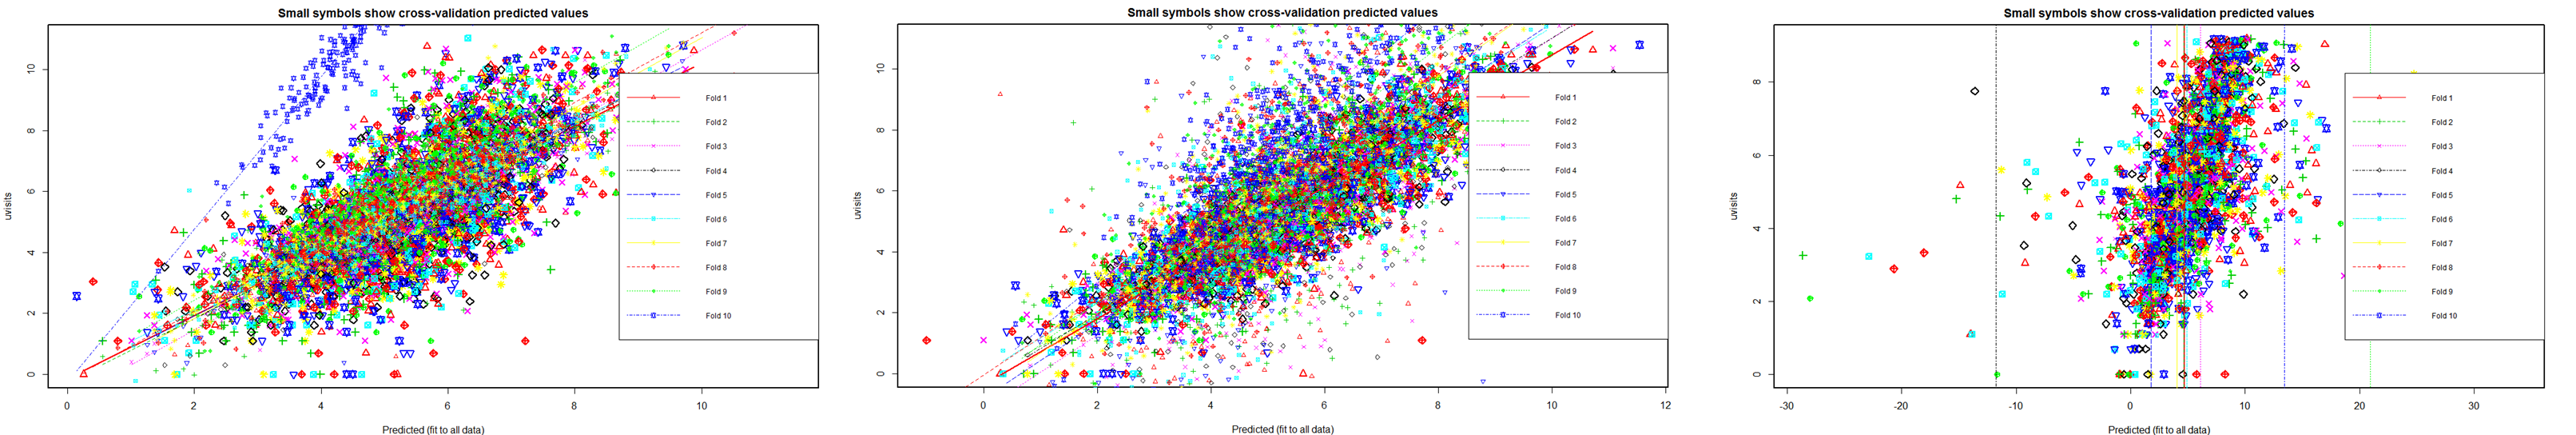
\includegraphics[width=1.0\textwidth]{proc.png}
  \caption{Obrázok znázorňuje postupnosť vývoju chýb pri pridávaní viac slov do modelu. Postupnosť je znázorňená pre počet 106 slov v modeli, 2649 slov a 4526 slov. }  
\end{figure}   	

Ako je vidieť z postupnosti na obrázku číslo 2 hlavný prúd, respektíve chyby sa viac rozptýlili pri pridaní väčšieho množstva slov do modelu. Toto do značnej miery pomohlo, ale za istou hranicou to už nebolo únosne. Preto sme tento postup označili ako slepú uličku a rozhodli sme sa vrátiť späť k najlepšiemu výsledku čo sme doposiaľ dosiahli, čo bolo pri počte 2649 slov v modeli a pokračovať iným smerom.

Ako prvý problém sme identifikovali outlaiery, teda články, ktoré sú počas dňa najviac čítane a svojou popularitou vyčnievali od zvyšku článkov. Približne každý deň sa vydá 10 takýchto článkov z celkového počtu v priemere 400 článkov za jeden deň. Takéto články nám značne zhoršovali výsledok a preto bolo jedným zo zaujímavých riešení ako sa s nimi vysporiadať ich odstránenie z predikčného modelu.

Pozorovaním čítanosti a ich zobrazením v histograme sme sa rozhodli odstrániť všetky články z čítanosťou nad 10 000. Takýchto článkov bolo celkom 141. Z celkového počtu článkov 4196 nám teda zostalo 4055. Výsledky po tejto úprave je vidieť v tabuľke číslo 2.


\begin{table}
\begin{center}
	\begin{tabular}{|p{5cm}|c|c|c|}
	\hline
	Vstupné atribúty & CV & Priemerná chyba & Medián chyby \\ \hline \hline
	2649 slov & 7.6 & 438 & 73.6 \\ \hline
	2649 slov, dĺžka článku & 7.41 & 434 & 72.6 \\ \hline
	2649 slov, dĺžka článku, kategória & 7.1 & 421 & 69.3 \\ \hline
	2649 slov, dĺžka článku, kategória, sekcia & 6.89 & 410 & 67.5  \\ \hline
	2649 slov, dĺžka článku, kategória, sekcia, čas & 7.12 & 434 & 70.5 \\ \hline
	\end{tabular}
\end{center}
\caption{Tabuľka znázorňuje výsledky pre 4055 článkov s postupným pridávaním atribútov do viacnásobnej lineárnej regresie. }
\end{table}

Ako je vidieť z tabuľky číslo 1 a 2 odstránením slov sme dosiahli značne zlepšenie, čo avšak nie je prekvapujúce. Priemerná chyba bola pred odstránením slov 909 po odstránení slov je 438. Medián bol 88,1 po odstránení je 73,6. Z týchto výsledkov len vyplýva, že sme si upravili štatistiku, ale nie samotný predikčný model.
  
Ďalšie experimenty sme zmerali na pridávanie nových atribútov do modelu. Ako je vidieť z tabuľky číslo 2 v prvom stĺpci sú uvedené nové atribúty, ktoré sme do modelu pridali. Pri prvom experimente takéhoto typu sme pridali dĺžku článkov, respektíve počet slov v ich texte. Táto úprava modelu bola úspešná a predikcia sa nám o málo zlepšila.

Ďalšiu úpravou bolo pridanie názvu kategórie, v ktorej sa článok nachádza na koniec každého textu článku. Takýto text sme znovu spracovali v metóde TF-IDF a potom sme znovu vybrali iba tie najdôležitejšie slová. Táto zmena nám značne pomohla a preto sme sa rozhodli podobným postupom pridať aj názov sekcie a opäť to pomohlo.

Poslednou, avšak nie až tak úspešnou úpravou bolo pridanie aspektu času vydania článku. Do modelu sme pridali ako nový nominálny atribút, hodinu vydania, týždeň vydania, deň vydania a deň vydania slovom, ktorý sme podobne ako v predchádzajúcich prípadoch pridali na koniec textu. Táto úprava nám značne zhoršila výsledok a preto sme ju označili ako ďalšiu slepú uličku.

\begin{figure}[h!]
  \centering  
      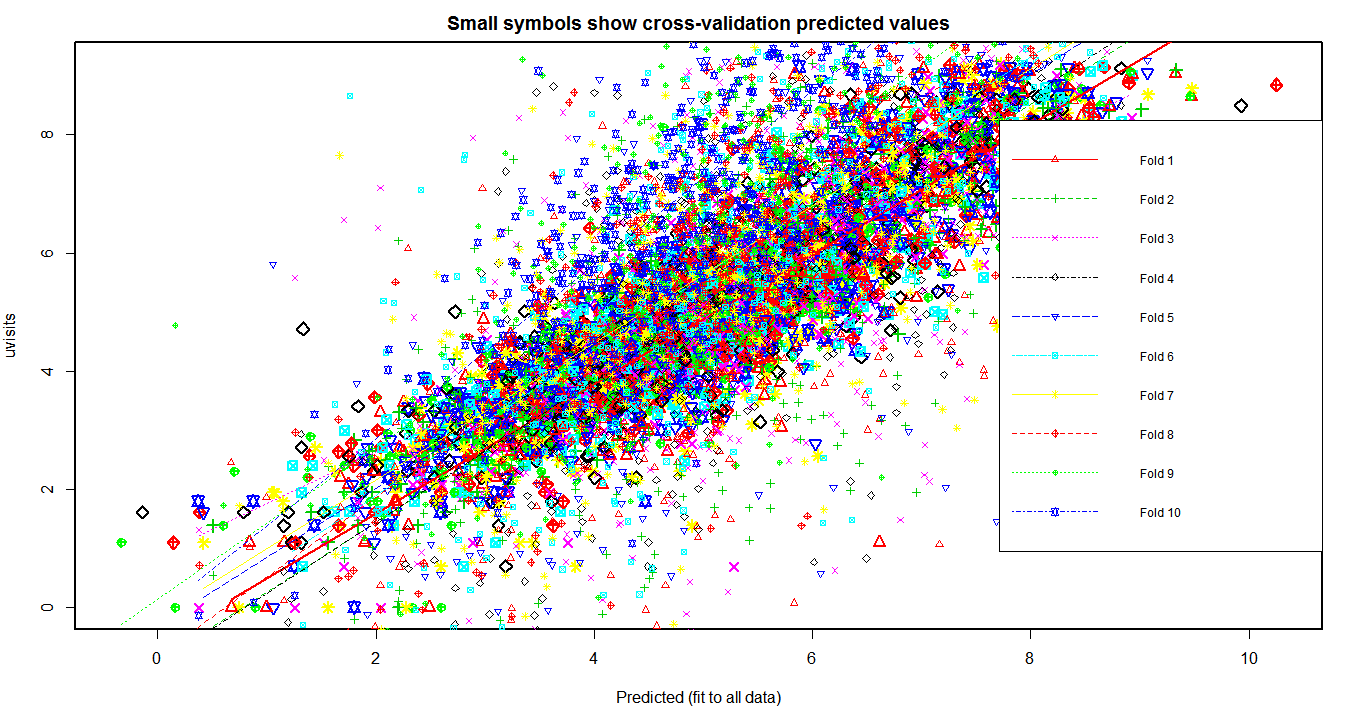
\includegraphics[width=1.0\textwidth]{plot11.png}
  \caption{Obrázok znázorňuje najlepšiu konfiguráciu atribútov(2649 slov, dĺžka článku, kategória, sekcia), ktorú sme s modelom dosiahli. }  
\end{figure} 

Najlepším výsledkom, ktorý sme dosiahli bola kombinácia atribútov 2649 slov spolu s dĺžkou článku, kategóriou a sekciou článku, ktorú je vidieť na obrázku číslo 3. Priemerná chyba tejto kombinácie bola 410 a medián chyby bol 67.5, čo v porovnaní so začiatočnou hodnotou je rázne zlepšenie.

\section{Záver} 
Predikcia popularity článkov je komplexná úloha a v našej práci sme sa jej dotkli len veľmi letmo. Je treba rozlíšiť či chcem predpovedať čitanosť všetkých článkov alebo len istej skupiny článkov, ktorá vyčnieva alebo naopak je nevýrazná. Zaujímavou úlohou by mohol byť hľadanie článkov, ktoré majú veľkú čitanosť, teda outlaierov. Keby sme vedeli podľa textu rozdeliť články na dve kategórie (napr. populárne a menej populárne), tak by sme vedeli upraviť predikčné modely na všetky kategórie, pre ktoré by to bolo potrebné a tak predikovať lepšie výsledky.

Model by sa dal zlepšiť aj nahradením súčasnej reprezentácie slov, ktorá je vytvorená  pomocou TF-IDF, za inú reprezentáciu vytvorenou pomocou neurónových sieti a učenia reprezentácie. Takéto reprezentácia by možno dokázala zachytiť lepšie vzťahy medzi slovami a poskytla by iné pohľady na dáta. 

Poslednou, ale taktiež významnou úpravou by mohlo byť analyzovanie vývoju článkov v čase a určovanie dôležitých slov v texte, ktoré značne odlišujú text od iného textu (angl. topic modeling). Takéto a iné nové formy atribútov v regresnom modely by mohli pomôcť určiť presnejšiu popularitu článkov.  



\begin{thebibliography}{7}
  \bibitem{diplomovka} Sopko, Pavol, Odporúčanie novinových článkov zohľadňujúce externý kontext používateľa, 2014, FIIT STU Bratislava
  \bibitem{pulse} Bandari, Roja; Asur, Sitaram; Huberman, Bernardo A., The Pulse of News in Social Media : Forecasting Popularity, ICWSM 2012, AAAI Press
  \bibitem{topic} Toraman, Cagri, News Selection with Topic Modeling, Fifth BCS-IRSG Symposium on Future Directions in Information Access (FDIA 2013)
\end{thebibliography}
\end{document}
